% ===========================================================================
% Detecting Face-Swap Deepfakes by Verifying Skeletal Gait Dynamics
% ISM 2026 submission (IEEE International Symposium on Multimedia)
%
% Build (from this directory):  latexmk -pdf ism_paper.tex
%
% Retargeted from the IEEEtran [journal] original. All technical claims and
% numbers are identical to paper/deepfake_paper.tex; see ../changelog.md.
%
% ANONYMIZATION: ISM 2026 publishes no review-mode policy (see
% ../requirements.md S3). Built single-blind. To anonymize, change the line
% \ismanonfalse  ->  \ismanontrue
% ===========================================================================

\documentclass[conference]{IEEEtran}

\newif\ifismanon
\ismanonfalse      % <-- set to \ismanontrue if ISM confirms double-blind review

\usepackage[utf8]{inputenc}
\usepackage[T1]{fontenc}
\usepackage{amsmath,amssymb,amsfonts}
\usepackage{graphicx}
\usepackage{booktabs}
\usepackage{array}
\usepackage{algorithm}
\usepackage{algorithmic}
\usepackage{url}
\usepackage{cite}
\usepackage{tikz}
\usepackage[colorlinks=true,linkcolor=blue!50!black,citecolor=blue!50!black,urlcolor=blue!50!black]{hyperref}
% NB: the installed pgf predates arrows.meta, so the legacy `arrows' library is used.
\usetikzlibrary{arrows,positioning,calc,fit,backgrounds,shapes.geometric}

% Float packing: LaTeX's defaults strand text when wide floats are present.
% These only change placement, never content.
\setcounter{topnumber}{3}
\setcounter{bottomnumber}{2}
\setcounter{totalnumber}{4}
\renewcommand{\topfraction}{0.92}
\renewcommand{\bottomfraction}{0.75}
\renewcommand{\textfraction}{0.07}
\renewcommand{\floatpagefraction}{0.75}
\renewcommand{\dbltopfraction}{0.92}
\renewcommand{\dblfloatpagefraction}{0.75}

\graphicspath{{figures/}}
\hyphenation{deep-fake deep-fakes bio-mech-an-i-cal}
\newcommand{\tabhead}[1]{\textbf{#1}}
\renewcommand{\arraystretch}{0.96}
\setlength{\textfloatsep}{6pt plus 2pt minus 2pt}
\setlength{\dbltextfloatsep}{6pt plus 2pt minus 2pt}
\setlength{\floatsep}{6pt plus 2pt minus 2pt}
\setlength{\abovecaptionskip}{2pt}

\begin{document}

\title{Detecting Face-Swap Deepfakes by Verifying\\Skeletal Gait Dynamics}

\ifismanon
  \author{\IEEEauthorblockN{Anonymous Submission}
          \IEEEauthorblockA{Paper ID: XXXX}}
\else
  \author{\IEEEauthorblockN{Arhaan Penwala, Abhishek Arun Raja Kodeeswaran,
          Aditya Bharti, Vibhav Sharma, and Deepika Roselind Johnson}
  \IEEEauthorblockA{School of Computer Science and Engineering\\
  Vellore Institute of Technology, Chennai Campus, India}}
\fi

\maketitle

% ===========================================================================
\begin{abstract}
Face-swap generators synthesise a face and composite it back into an otherwise
unmodified frame. The body they leave behind still walks the way the source
person walks. We verify the claimed identity against the one signal the
generator never touches. Our system extracts a 78-dimensional skeletal gait descriptor
per frame---hip-centred coordinates, six joint flexion angles and velocities
over 12 biomechanically selected MediaPipe landmarks---and classifies the
per-timestep discrepancy against the claimed identity's enrolled signature with
a temporal convolutional verification network. On GaitDeepfake-13, a
13-subject corpus of 66 walking videos expanded to 1{,}056 by augmentation,
under strict leave-one-subject-out cross-validation, it attains a pooled
ROC-AUC of $94.95\%$ over 2{,}240 verification pairs (per-fold
$95.10\% \pm 3.08\%$), accuracy $87.04\% \pm 3.65\%$ and an equal error rate of
$12.27\% \pm 3.80\%$. Gradient attribution rests the decision on shoulder
countermotion and distal heel-strike kinematics, with joint angles carrying
$1.94\times$ their proportional share despite occupying 6 of 78 dimensions. On
three FaceFusion-generated face-swaps the system rejected the claimed identity
in all three cases and matched the true body source above $0.9998$
similarity---an existence check, not a powered claim. An ablation over 13 folds
and 3 seeds finds that adding a CNN, BiLSTM or Transformer encoder to the
decision path costs $2.5$ to $5.9$ ROC-AUC points (all $p < 10^{-3}$, paired),
so the network's simplicity is a result rather than a concession.
\end{abstract}

\begin{IEEEkeywords}
Media forensics, multimedia security, deepfake detection, gait analysis,
behavioural biometrics, identity verification, pose estimation, explainable AI.
\end{IEEEkeywords}

% ===========================================================================
\section{Introduction}
\label{sec:intro}

The dominant paradigm in video deepfake detection looks for evidence of
manipulation inside the manipulated region: detectors learn blending
boundaries, frequency-domain irregularities, warping residues and temporal
flicker in and around the face crop~\cite{recce,multi_attn,ftcn,altfreezing,%
fsbi}. The paradigm is productive and structurally fragile at once, because it
places the detector in direct opposition to the generator's objective. Every
improvement in synthesis quality erodes precisely the signal the detector
depends on, which is why cross-dataset generalisation remains the field's most
stubborn problem---methods approaching saturation within a training corpus lose
substantial ground on unseen manipulations and
generators~\cite{recce,ftcn,deepfake_eval}.

We take the opposite stance: instead of interrogating the region the adversary
controls, we interrogate a region the adversary does not modify at all. The
observation is mechanical rather than statistical. Contemporary face-swap
pipelines---FaceFusion with InSwapper~\cite{facefusion,insightface},
SimSwap~\cite{simswap} and their descendants---detect a face, synthesise a
replacement, and composite it back through a mask confined to the facial
region, carrying the torso, limbs and background through from the source
footage modulo recompression. A face-swapped video of person $B$ built on
footage of person $A$ therefore contains $B$'s face and $A$'s \emph{gait}. Human
locomotion is constrained by skeletal proportion, mass distribution and
individual motor control, and is a well-established biometric in its own
right~\cite{gaitgraph,gaitpt,gaitformer,perry_gait,winter_biomech}: the forgery
carries, in plain sight, an identity signal contradicting its own claim.

\subsection{Problem Formulation}

We treat detection as identity verification rather than binary artefact
classification. Given a video $V$ and a claimed identity $I_c$ drawn from an
enrolled gallery, the system computes
\begin{equation}
f(V, I_c) \rightarrow
\begin{cases}
\textsc{authentic} & \text{if the gait in } V \text{ matches } I_c,\\
\textsc{deepfake}  & \text{otherwise.}
\end{cases}
\label{eq:problem}
\end{equation}

Consequently the system detects an \emph{identity inconsistency}, not the
presence of synthesis. It
requires an enrolled reference and will not flag a wholly synthetic person with
no claimed identity. Section~\ref{sec:discussion} returns to what this rules in
and out.

\subsection{Contributions}

\begin{enumerate}
\item A \textbf{gait-based verification formulation} of face-swap detection
      whose discriminative signal lies outside the generator's output support
      (Section~\ref{sec:method}).
\item A \textbf{difference-based temporal verification network} that compares
      sequences before pooling, avoiding the representation collapse a Siamese
      formulation suffers at this corpus size (Section~\ref{sec:verifier}).
\item A \textbf{subject-disjoint evaluation} over 13 leave-one-subject-out
      folds and 2{,}240 verification pairs, with per-fold dispersion and two
      operating points (Sections~\ref{sec:setup}--\ref{sec:results}).
\item \textbf{Gradient attribution over the skeleton}, quantifying the
      disproportionate value of the six joint-angle dimensions
      (Section~\ref{sec:explain}).
\item \textbf{An ablation that refutes the alternative}: adding a CNN, BiLSTM or
      Transformer stack costs $2.5$ to $5.9$ ROC-AUC points (all
      $p < 10^{-3}$, paired), and removing the raw comparison collapses
      performance to chance (Section~\ref{sec:ablation-results}).
\end{enumerate}

% ===========================================================================
\section{Related Work}
\label{sec:related}

\subsection{Face-Based Deepfake Detection}

Detection of facial manipulation has converged on spatial artefact modelling,
temporal coherence modelling, or a hybrid. Multi-attentional
detection~\cite{multi_attn} treats forgery as fine-grained classification. RECCE~\cite{recce} uses reconstruction error of genuine faces
as the forgery cue, observing that earlier methods degrade towards
approximately $60\%$ AUC on unseen data and reporting roughly $70.9\%$
cross-dataset AUC on Celeb-DF-v2. FTCN~\cite{ftcn} removes spatial convolution
capacity to force reliance on temporal incoherence, reaching roughly
$86$--$89\%$ AUC on Celeb-DF cross-dataset, and
AltFreezing~\cite{altfreezing} alternately freezes spatial and temporal weights
in a 3D ConvNet for $89.5\%$ on the same setting; FSBI~\cite{fsbi} synthesises
training forgeries via frequency-enhanced self-blending. In-corpus performance
is near saturated while cross-corpus performance is not, and the gap is
generator-dependent. Our approach is complementary rather than competitive: it
never examines the facial region, so its failure modes are uncorrelated with
every method here.

\subsection{Skeleton-Based Gait Recognition}

Model-based gait recognition operates on pose sequences rather than
silhouettes, conferring robustness to clothing and carried objects.
GaitGraph~\cite{gaitgraph} applies graph convolution to skeleton sequences;
GaitPT~\cite{gaitpt} reaches $82.6\%$ average accuracy on CASIA-B from
skeletons alone; GaitFormer~\cite{gaitformer} reports $92.5\%$ on CASIA-B after
multi-task pretraining. Skeletal kinematics thus carry sufficient identity
information for recognition at scale; we redirect that premise to adjudicating a
specific claimed identity, a verification problem with its own metric
conventions~\cite{iso19795}.

\subsection{Behavioural and Whole-Body Forgery Detection}

Behavioural biometrics entered deepfake detection with Agarwal
\emph{et al.}~\cite{agarwal2019}, who modelled correlations among facial action
units and head motion, later extending beyond the face to gestural and vocal
mannerisms~\cite{agarwal_pnas}. Attention has since moved to the whole
body. Human Action CLIPs~\cite{humanactionclips} detects AI-generated human
motion; TT-DF~\cite{ttdf} benchmarks human body forgery detection from pose and
motion inconsistency; Chapariniya \emph{et al.}~\cite{convkeypoints} identify
people from whole-body conversational keypoints, framed against
face-reenactment threats. Closest to this work, DeAndres-Tame
\emph{et al.}~\cite{gaitfidelity} evaluate whether generative human-animation
models preserve gait identity cues and find that they do not---an evaluation
study rather than a deployed detector, but one that independently supports our
premise.

\subsection{Positioning}

Under-explored is \emph{locomotion gait-cycle skeletal dynamics as the primary discriminative feature} for verifying a claimed identity in a face-swapped video under a subject-disjoint protocol. The nearest work~\cite{gaitfidelity} measures gait fidelity in generated animation without building a detector; the nearest detectors~\cite{ttdf,humanactionclips} target whole-body synthesis, not face-swap, where the body is authentic and only the claim is false.

% ===========================================================================
\section{Proposed Method}
\label{sec:method}

\begin{figure*}[!t]
\centering
% ---------------------------------------------------------------------------
% Fig. 1 -- End-to-end verification pipeline and network architecture.
% Pure TikZ (vector). Replaces raster fig1_pipeline.png + fig4_architecture.png.
% Legacy-pgf compatible: uses the `arrows' library, not `arrows.meta'.
% Two-row layout: (top) feature extraction, (bottom) difference verification.
% ---------------------------------------------------------------------------
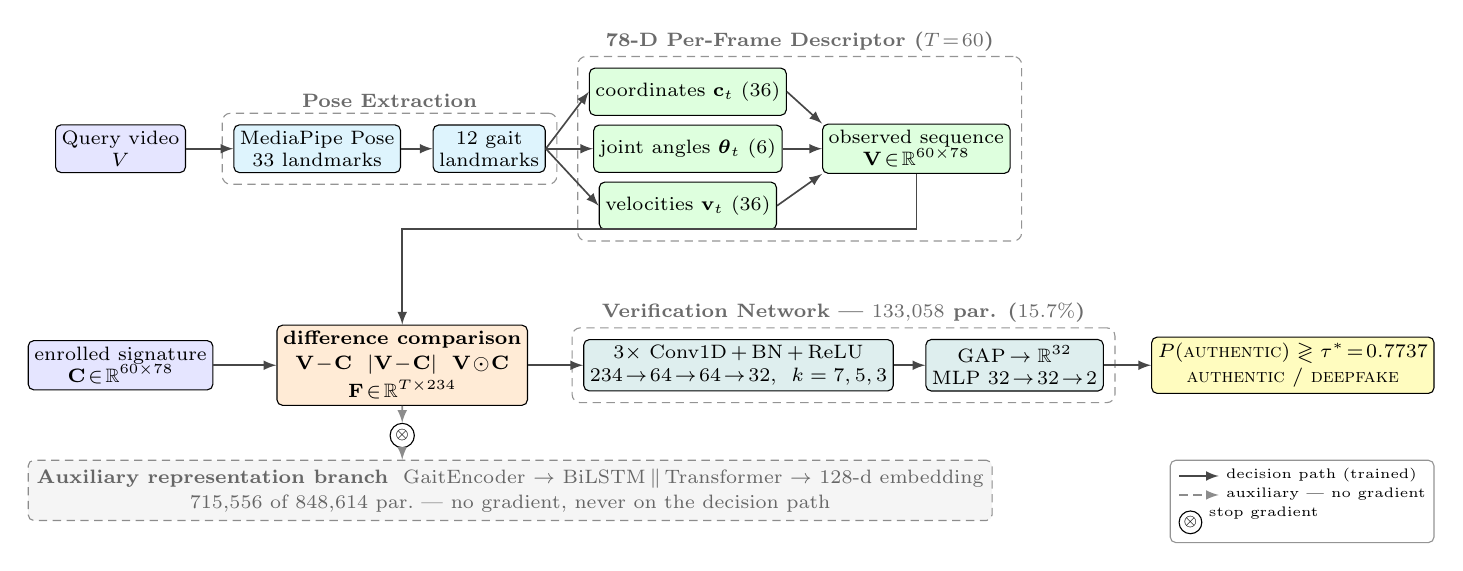
\begin{tikzpicture}[
  font=\scriptsize,
  blk/.style   = {draw, rounded corners=2pt, align=center, inner sep=2.2pt,
                  minimum height=6.0mm, line width=0.4pt},
  inp/.style   = {blk, fill=blue!10},
  pose/.style  = {blk, fill=cyan!13},
  feat/.style  = {blk, fill=green!13},
  comp/.style  = {blk, fill=orange!16},
  conv/.style  = {blk, fill=teal!13},
  head/.style  = {blk, fill=yellow!25},
  auxb/.style  = {draw=black!45, rounded corners=2pt, align=center, inner sep=3pt,
                  fill=black!4, densely dashed, text=black!60, line width=0.4pt},
  grp/.style   = {draw=black!42, densely dashed, rounded corners=3pt, inner sep=4pt},
  gl/.style    = {font=\scriptsize\bfseries, text=black!58, inner sep=1.5pt},
  ar/.style    = {-latex, semithick, black!72},
  arx/.style   = {-latex, semithick, black!45, densely dashed},
]

% =========================== ROW 1 : feature extraction ====================
\node[inp]                     (vid) at (0,0)   {Query video\\$V$};
\node[pose, right=6mm of vid]  (mp)             {MediaPipe Pose\\33 landmarks};
\node[pose, right=4mm of mp]   (kp)             {12 gait\\landmarks};

\node[feat, right=6mm of kp]   (an)             {joint angles $\boldsymbol{\theta}_t$ (6)};
\node[feat, above=1.1mm of an] (co)             {coordinates $\mathbf{c}_t$ (36)};
\node[feat, below=1.1mm of an] (ve)             {velocities $\mathbf{v}_t$ (36)};

\node[feat, right=5mm of an]   (vv)
  {observed sequence\\$\mathbf{V}\!\in\!\mathbb{R}^{60\times 78}$};

% =========================== ROW 2 : verification ==========================
\node[inp]  (sig) at (0,-2.75) {enrolled signature\\$\mathbf{C}\!\in\!\mathbb{R}^{60\times 78}$};

\node[comp, right=8mm of sig] (cmp)
  {\textbf{difference comparison}\\[0.4mm]
   $\mathbf{V}\!-\!\mathbf{C}$\ \ $|\mathbf{V}\!-\!\mathbf{C}|$\ \ $\mathbf{V}\!\odot\!\mathbf{C}$\\[0.3mm]
   $\mathbf{F}\!\in\!\mathbb{R}^{T\times 234}$};

\node[conv, right=7mm of cmp] (cnn)
  {$3\times$ Conv1D\,+\,BN\,+\,ReLU\\$234\!\to\!64\!\to\!64\!\to\!32$,\ \ $k=7,5,3$};

\node[conv, right=4mm of cnn] (gm)
  {GAP\,$\to\mathbb{R}^{32}$\\MLP $32\!\to\!32\!\to\!2$};

\node[head, right=6mm of gm] (verd)
  {$P(\textsc{authentic})\gtrless\tau^{\ast}\!=\!0.7737$\\[0.3mm]
   \textsc{authentic}\ /\ \textsc{deepfake}};

% =========================== main arrows ===================================
\draw[ar] (vid) -- (mp);
\draw[ar] (mp)  -- (kp);
\draw[ar] (kp.east) -- (co.west);
\draw[ar] (kp.east) -- (an.west);
\draw[ar] (kp.east) -- (ve.west);
\draw[ar] (co.east) -- (vv.north west);
\draw[ar] (an.east) -- (vv.west);
\draw[ar] (ve.east) -- (vv.south west);

% observed sequence drops into the comparison
\coordinate (br) at ($(vv.south)+(0,-7mm)$);
\draw[ar] (vv.south) -- (br) -| (cmp.north);
\draw[ar] (sig) -- (cmp);

\draw[ar] (cmp) -- (cnn);
\draw[ar] (cnn) -- (gm);
\draw[ar] (gm)  -- (verd);

% =========================== auxiliary branch ==============================
\node[auxb, anchor=north west] (aux)
  at ($(sig.west)+(0,-12mm)$)
  {\textbf{Auxiliary representation branch}\ \ GaitEncoder $\to$
   BiLSTM\,$\|$\,Transformer $\to$ 128-d embedding\\[0.4mm]
   $715{,}556$ of $848{,}614$ par.\ --- no gradient, never on the decision path};

\node[circle, draw, fill=white, inner sep=0.7pt, line width=0.4pt]
  (sg) at ($(cmp.south)!0.55!(cmp.south|-aux.north)$) {\tiny$\otimes$};
\draw[arx] (cmp.south) -- (sg);
\draw[arx] (sg) -- (cmp.south|-aux.north);

% =========================== group boxes ===================================
\begin{scope}[on background layer]
  \node[grp, fit=(mp)(kp), label={[gl]above:Pose Extraction}] {};
  \node[grp, fit=(co)(ve)(vv),
        label={[gl]above:78-D Per-Frame Descriptor ($T\!=\!60$)}] {};
  \node[grp, fit=(cnn)(gm),
        label={[gl]above:Verification Network --- $133{,}058$ par. ($15.7\%$)}] {};
\end{scope}

% =========================== legend ========================================
\node[draw=black!42, rounded corners=2pt, fill=white, inner sep=3pt,
      font=\tiny, align=left, anchor=north east]
  at ($(verd.east)+(0,-12mm)$)
  {\tikz[baseline=-0.5ex]{\draw[ar](0,0)--(5mm,0);}\ decision path (trained)\\[0.3mm]
   \tikz[baseline=-0.5ex]{\draw[arx](0,0)--(5mm,0);}\ auxiliary --- no gradient\\[0.3mm]
   \tikz[baseline=-0.5ex]{\node[circle,draw,inner sep=0.5pt,line width=0.4pt]{\tiny$\otimes$};}\ stop gradient};

\end{tikzpicture}

\caption{End-to-end verification pipeline. The observed sequence is compared
against the claimed identity's enrolled signature \emph{before} pooling, and a
three-stage temporal CNN classifies the $T\times234$ comparison tensor. The
auxiliary branch holds $715{,}556$ of the model's $848{,}614$ parameters but
receives no gradient and never reaches the decision path
(Section~\ref{sec:aux}).}
\label{fig:arch}
\end{figure*}

\subsection{Threat Model}
\label{sec:threat}

\begin{figure}[!tb]
\centering
% ---------------------------------------------------------------------------
% Fig. 2 -- Threat model: the asymmetry the method exploits.
% Pure TikZ (vector), sized for \columnwidth. Replaces raster fig2_threat_model.png.
% Legacy-pgf compatible: uses the `arrows' library, not `arrows.meta'.
% Grayscale-safe: the rewritten region is marked by a heavy dashed border and an
% explicit "(synthesised)" label, not by colour alone.
% ---------------------------------------------------------------------------
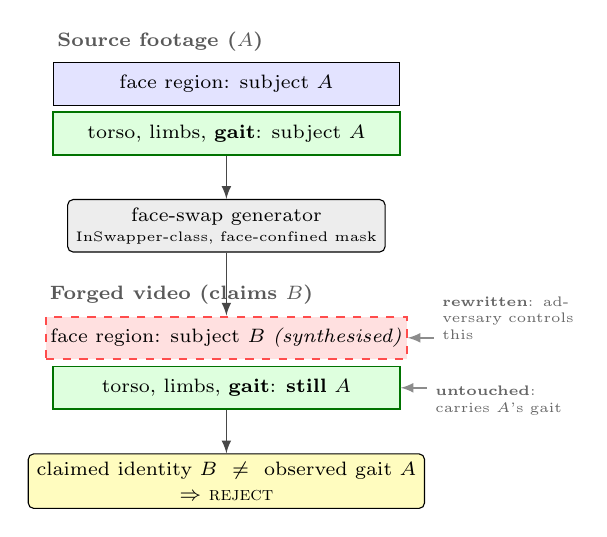
\begin{tikzpicture}[
  font=\scriptsize,
  band/.style   = {draw, align=center, minimum height=5.4mm, minimum width=44mm,
                   inner sep=1.5pt, line width=0.35pt},
  faceok/.style = {band, fill=blue!11},
  facebad/.style= {band, fill=red!12, draw=red!70, dashed, line width=0.7pt},
  body/.style   = {band, fill=green!13, draw=green!45!black, line width=0.7pt},
  gen/.style    = {draw, rounded corners=2pt, fill=black!7, align=center,
                   inner sep=3pt, line width=0.4pt},
  ar/.style     = {-latex, semithick, black!72},
  note/.style   = {font=\tiny, text=black!60, align=left, inner sep=1pt,
                   text width=17mm},
  capt/.style   = {font=\scriptsize\bfseries, text=black!65, inner sep=1.5pt},
]

% ----------------------------- source footage -----------------------------
\node[faceok] (sf) at (0,0) {face region: subject $A$};
\node[body, below=0.7mm of sf] (sb) {torso, limbs, \textbf{gait}: subject $A$};
\node[capt, anchor=south west] at ($(sf.north west)+(0,0.8mm)$)
  {Source footage ($A$)};

% ----------------------------- generator ----------------------------------
\node[gen, below=5.5mm of sb] (gen)
  {face-swap generator\\[-0.3mm]{\tiny InSwapper-class, face-confined mask}};
\draw[ar] (sb.south) -- (gen.north);

% ----------------------------- forged video -------------------------------
\node[facebad, below=8mm of gen] (ff)
  {face region: subject $B$ \textit{(synthesised)}};
\node[body, below=0.7mm of ff] (fb) {torso, limbs, \textbf{gait}: \textbf{still} $A$};
\node[capt, anchor=south west] at ($(ff.north west)+(0,0.8mm)$)
  {Forged video (claims $B$)};
\draw[ar] (gen.south) -- (ff.north);

% ----------------------------- side annotations ---------------------------
\node[note, anchor=south west] (n1) at ($(ff.east)+(4mm,-0.6mm)$)
  {\textbf{rewritten}: adversary controls this};
\node[note, anchor=north west] (n2) at ($(fb.east)+(4mm,0.6mm)$)
  {\textbf{untouched}: carries $A$'s gait};
\draw[semithick, black!45, latex-] (ff.east) -- ($(ff.east)+(3.4mm,0)$);
\draw[semithick, black!45, latex-] (fb.east) -- ($(fb.east)+(3.4mm,0)$);

% ----------------------------- verdict ------------------------------------
\node[draw, rounded corners=2pt, fill=yellow!25, align=center, inner sep=3pt,
      line width=0.4pt, below=5.5mm of fb] (ver)
  {claimed identity $B$\ \ $\neq$\ \ observed gait $A$\\[0.3mm]
   $\Rightarrow$ \textsc{reject}};
\draw[ar] (fb.south) -- (ver.north);

\end{tikzpicture}

\caption{The asymmetry the method exploits. The generator rewrites only the
face-confined band, so a forgery claiming subject~$B$ still walks with
subject~$A$'s gait. The generator never models locomotion, so this
inconsistency is structural, not an artefact better synthesis will remove.}
\label{fig:threat}
\end{figure}

We assume an adversary who produces a face-swapped video: a genuine recording
of a source subject with a target subject's face composited into the facial
region, presented under the target's identity. The adversary may use any
face-swap model and any face-enhancement post-process, and may recompress the
result, but does \emph{not} re-synthesise or retime body motion.

Under this model the detector's task reduces to Eq.~\ref{eq:problem}, and its
robustness has an unusual character: it is invariant to the quality of the face
swap, because it never observes the swapped region (Fig.~\ref{fig:threat}).
Section~\ref{sec:threats} discusses adversaries violating the last assumption.

\subsection{Dataset}
\label{sec:dataset}

Evaluation uses GaitDeepfake-13~\cite{gaitdeepfake13}, collected for this work.
Thirteen subjects were recorded walking at natural pace in controlled indoor
conditions, from frontal and side viewpoints, yielding 66 original recordings
(3--5 per subject) at 30\,fps and 720p--1080p. Subjects were students aged
approximately 19--25 of both sexes. Augmentation expands the corpus to
1{,}056 sequences; each is resampled to $T = 60$ frames ($\approx$2\,s) of
78-dimensional descriptors. The corpus also contains 3 face-swapped test clips
(FaceFusion / InSwapper), and the leave-one-subject-out protocol yields 2{,}240
verification pairs, of which 1{,}120 are genuine.

Each recording was expanded $16	imes$ ($66 	imes 16 = 1{,}056$) by transformations that leave the skeletal trajectory unchanged: photometric (blur, brightness $\pm0.2$--$0.3$, contrast, colour jitter, grayscale, noise), anatomically plausible geometric (flip, rotation $\le10^{\circ}$, zoom), and temporal (speed $0.8	imes$/$1.2	imes$, reversal, exploiting the approximate time-reversal symmetry of the gait cycle~\cite{perry_gait}), plus a combined pass.

\subsection{Pose Estimation and Feature Extraction}
\label{sec:features}

Pose is estimated with MediaPipe Pose Landmarker~\cite{mediapipe}
(\texttt{pose\_landmarker\_lite}, FP16, per-frame IMAGE mode, detection and
tracking confidence $0.5$), producing 33 three-dimensional landmarks per frame.
We retain 12: the bilateral shoulders, hips, knees, ankles, heels and foot
indices. The selection is driven by gait
biomechanics~\cite{perry_gait,winter_biomech}---the lower-limb
chain from hip through knee, ankle, heel and foot index spans the events that
define the gait cycle (heel strike, stance, toe-off), while the shoulders
capture the trunk countermotion that balances angular momentum during swing.
Facial, elbow and wrist landmarks are discarded; the facial ones on principle,
since they lie inside the region the adversary controls.

\begin{figure}[!tb]
\centering
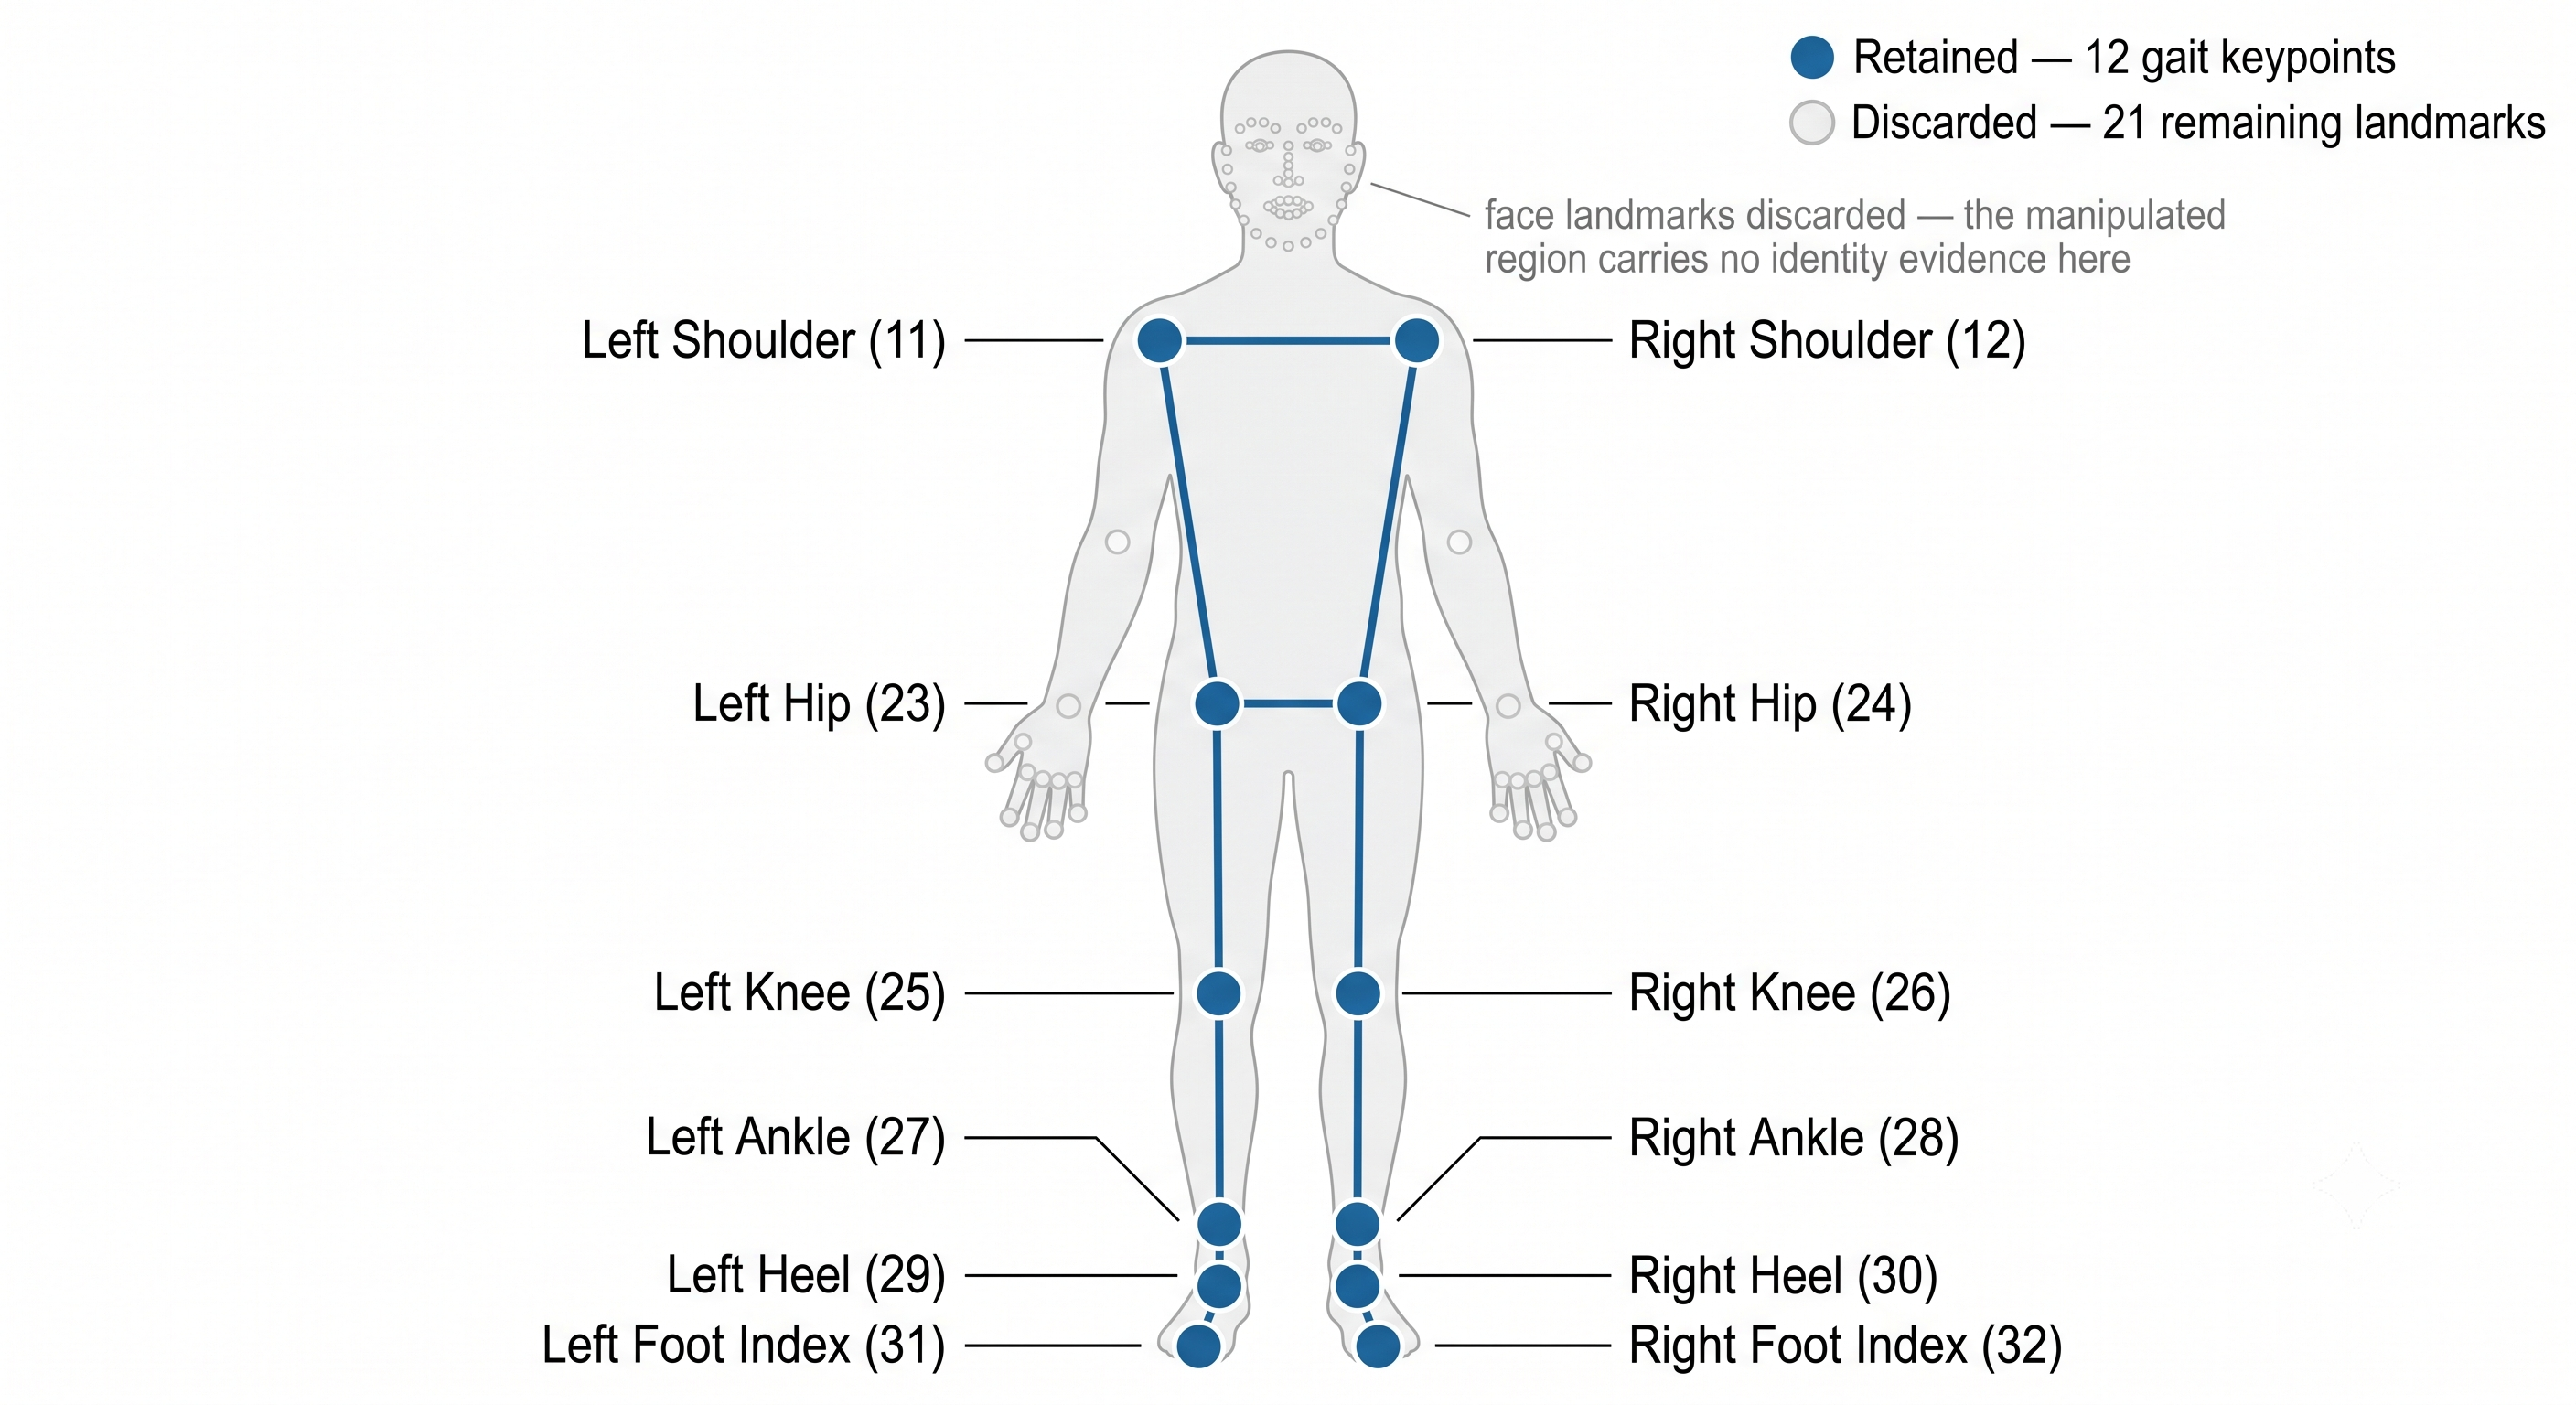
\includegraphics[width=\columnwidth]{fig3_keypoints.png}
\caption{The 12 retained gait keypoints (blue) of the 33 MediaPipe landmarks;
facial, elbow and wrist landmarks are discarded.}
\label{fig:keypoints}
\end{figure}

Video pose agrees with Vicon motion capture to within a few degrees (errors $4.0^{\circ}$--$7.4^{\circ}$ at hip, knee, ankle~\cite{stenum2021}), though that study used OpenPose, not MediaPipe.

For frame $t$ the descriptor concatenates three blocks, $\mathbf{f}_t = \left[\, \mathbf{c}_t \;\|\; \boldsymbol{\theta}_t \;\|\; \mathbf{v}_t \,\right] \in \mathbb{R}^{78}$.
\emph{Normalised coordinates} $\mathbf{c}_t \in \mathbb{R}^{36}$ are the 12
landmark positions re-expressed relative to the pelvis centre, $\hat{\mathbf{p}}_i^{(t)} = \mathbf{p}_i^{(t)} - \tfrac{1}{2}\left(\mathbf{p}_{\text{L\_Hip}}^{(t)} + \mathbf{p}_{\text{R\_Hip}}^{(t)}\right), \; i = 1,\dots,12$, removing translation and much of the scale variation induced by camera
distance~\cite{gaitgraph,gaitpt}. \emph{Joint angles}
$\boldsymbol{\theta}_t \in \mathbb{R}^{6}$ are three-point flexion angles
\begin{equation}
\theta_{abc} = \arccos\!\left(
\frac{(\mathbf{p}_a - \mathbf{p}_b) \cdot (\mathbf{p}_c - \mathbf{p}_b)}
{\lVert \mathbf{p}_a - \mathbf{p}_b \rVert \,
 \lVert \mathbf{p}_c - \mathbf{p}_b \rVert}\right),
\end{equation}
evaluated as $\theta(\text{hip},\text{knee},\text{ankle})$,
$\theta(\text{shoulder},\text{hip},\text{knee})$ and
$\theta(\text{knee},\text{ankle},\text{foot})$ bilaterally; they are scale-free
by construction and encode biomechanical constraint directly. \emph{Velocities}
$\mathbf{v}_t = \mathbf{c}_t - \mathbf{c}_{t-1} \in \mathbb{R}^{36}$ are
first-order differences with $\mathbf{v}_1 = \mathbf{0}$, capturing the rate
structure of the gait cycle.

Sequences are resampled to $T = 60$ frames---longer uniformly subsampled,
shorter zero-padded, clips with fewer than 10 valid frames rejected---spanning
roughly two seconds at 30\,fps, or one to two complete gait
cycles~\cite{perry_gait}. Each dimension is then z-score normalised,
$\hat{f}_j = (f_j - \mu_j)/\max(\sigma_j, 10^{-6})$, since the blocks occupy
incommensurate scales.

\subsection{Identity Enrolment}
\label{sec:enrollment}

Each identity $I$ is enrolled by averaging the descriptors of its original
(non-augmented) recordings per timestep,
\begin{equation}
\bar{\mathbf{f}}_t^{(I)} = \frac{1}{|V_I|}\sum_{v \in V_I} \mathbf{f}_t^{(v)},
\qquad t = 1,\dots,60,
\end{equation}
yielding a $60 \times 78$ signature per subject. Averaging suppresses per-take
noise while preserving the subject's characteristic temporal profile. The
signature is used as a full sequence, not collapsed to a vector---the
verification network consumes it as a second input stream.

\subsection{Verification Network}
\label{sec:verifier}

The network classifies the discrepancy between the observed sequence
$\mathbf{V} \in \mathbb{R}^{T \times 78}$ and the claimed identity's signature
$\mathbf{C} \in \mathbb{R}^{T \times 78}$ directly, without first reducing
either to a pooled embedding. Three per-timestep comparison signals are
concatenated,
\begin{equation}
\mathbf{F} = \left[\, (\mathbf{V}-\mathbf{C}) \;\|\;
|\mathbf{V}-\mathbf{C}| \;\|\;
(\mathbf{V} \odot \mathbf{C}) \,\right] \in \mathbb{R}^{T \times 234},
\end{equation}
where the signed difference localises \emph{where} and \emph{in which
direction} the sequences diverge, the absolute difference supplies magnitude
invariant to sign, and the elementwise product responds where the two agree.
$\mathbf{F}$ is transposed to channel-first order and passes through three 1D
convolutional stages with decreasing receptive fields ($234 \rightarrow 64$,
$k=7$; $64 \rightarrow 64$, $k=5$; $64 \rightarrow 32$, $k=3$), each with batch
normalisation and ReLU, and dropout on the first two. Global average pooling
over time yields a 32-dimensional summary, which a two-layer MLP
($32 \rightarrow 32 \rightarrow 2$) maps to two logits. The verdict score is
$P(\textsc{authentic}) = \mathrm{softmax}(\cdot)_1$.

\subsubsection{Why differences rather than embedding distances}
Our initial design followed the standard Siamese template: encode both
sequences with shared weights, pool to embeddings, score their distance. On
this corpus it collapsed---the encoder converged to a near-constant embedding,
driving all pairwise distances towards a single value and the classifier
towards the majority prediction. With 13 identities and a per-timestep
signature that is itself an average of few recordings, pooling discards
precisely the fine temporal structure separating individuals. Comparing
sequences before pooling avoids this: discriminative information is preserved
at full temporal resolution, and the pooling that remains happens after the
comparison, on evidence rather than identity.
Section~\ref{sec:ablation-results} tests this directly.

\subsubsection{Auxiliary representation branch}
\label{sec:aux}
The trained checkpoint also contains a representation branch retained from the
Siamese design and used for enrolment analysis and diagnostics: a residual 1D
CNN encoder ($78 \rightarrow 64 \rightarrow 128$) feeding a dual-path temporal
model whose BiLSTM ($h=64$, bidirectional) and Transformer encoder
($d_{\text{model}}=128$, 4 heads, 2 layers) are fused into a 128-dimensional
embedding.

This affects how Section~\ref{sec:results} should be read. Under the cross-entropy objective
applied to the verification logits, gradients reach only the pairwise-comparison
path; the representation branch receives no learning signal from the training
objective. Of the model's $848{,}614$ parameters, $133{,}058$ ($15.7\%$) lie on
the decision path---$131{,}936$ in the temporal CNN and $1{,}122$ in the
classifier MLP. All quantitative results below are therefore properties of the
difference-based verification network, not of the CNN--BiLSTM--Transformer
stack. Section~\ref{sec:ablation-results} asks whether that stack \emph{should}
be connected, and finds that it should not.

\subsection{Training}
\label{sec:training}

Training pairs are sampled with a $50/50$ balance: half pair a video with its
own identity's signature (label \textsc{authentic}), half with a uniformly
sampled different identity's signature (label \textsc{deepfake}). This
simulates the identity-mismatch condition a face swap induces and prevents the
degenerate constant-prediction solution. Optimisation uses
AdamW~\cite{adamw} at $10^{-3}$ with weight decay $10^{-4}$, batch size 16,
gradient-norm clipping at $1.0$, dropout $0.1$, and
\texttt{ReduceLROnPlateau} (factor $0.5$, patience 7). Early stopping monitors
validation accuracy with patience 20 and $\delta_{\min} = 10^{-3}$. The loss is class-weighted
cross-entropy over a maximum of 50 epochs (30 under LOOCV), on an NVIDIA RTX
3050 (6\,GB, CUDA 12.4). The single-split reference model reached $93.92\%$
validation accuracy at epoch 46 against $98.38\%$ training accuracy.

% ===========================================================================
\section{Experimental Setup}
\label{sec:setup}

\subsection{Leave-One-Subject-Out Cross-Validation}

The primary protocol is 13-fold leave-one-subject-out cross-validation. In fold
$k$, every recording of subject $s_k$---original and all 15
augmentations---is withheld, normalisation statistics are recomputed from the
remaining 12 subjects, those 12 identities are re-enrolled from the training
split alone, and a model is trained from scratch for 30 epochs before being
evaluated on the held-out subject's balanced genuine/impostor pairs.

Subject-level rather than video-level partitioning is a requirement, not a
refinement: because augmented clips derive from originals, a video-level split
would place 15 near-duplicates of a test clip into training and yield an
estimate with no bearing on unseen subjects. LOOCV suits small-cohort biometric
evaluation~\cite{iso19795}, with the caveat that its variance is high at this
cohort size~\cite{varoquaux_small}. The full 13-fold procedure took
1{,}228\,s.

\subsubsection{A protocol detail, stated up front}
\label{sec:transductive}
The evaluation script producing our headline LOOCV figures normalises the
held-out subject using that subject's own statistics rather than the training
split's---a transductive choice, not the one a strict reading of the protocol
implies. We measured what it is worth by running the deployed model both ways
across all 13 folds: training statistics yield $94.67\% \pm 3.06\%$ ROC-AUC
against $94.97\% \pm 2.90\%$ for the shipped behaviour, a difference of $0.30$
points that is not significant ($p = 0.73$, paired, $n = 13$). The headline
result is therefore insensitive to this choice, and all ablation comparisons
use training statistics throughout.

\subsection{Metrics and Operating Points}

We report ROC-AUC as a threshold-free measure of separability~\cite{fawcett_roc};
equal error rate, the biometric convention~\cite{iso19795}; and accuracy,
precision, recall and F1 at an explicit operating point.

Two aggregation modes are reported. The \emph{per-fold} statistic is the mean
and standard deviation of a metric computed within each of the 13 folds
(variation by subject); the \emph{pooled} statistic is computed once over all
2{,}240 scores (behaviour on the population). They differ---pooled AUC is
$94.95\%$ against a per-fold mean of $95.10\%$---because folds carry unequal
sample counts and pooling forces one global ranking across models trained on
different splits. Two operating points are likewise reported: the native
$\tau = 0.5$ argmax decision, at which the per-fold metrics of
Table~\ref{tab:perfold} were computed, and the deployed threshold chosen by
Youden's $J$~\cite{youden},
$\tau^* = \arg\max_\tau [\mathrm{TPR}(\tau) - \mathrm{FPR}(\tau)]$, on the
pooled LOOCV ROC, giving $\tau^* = 0.7737$ with $\mathrm{TPR} = 83.57\%$,
$\mathrm{FPR} = 8.48\%$ and $J = 0.7509$.

\subsection{Ablation and Face-Swap Protocols}

Five variants were trained under the full LOOCV protocol at three random seeds,
differing only in how the observed and claimed sequences are encoded before
comparison. All share folds, seeds, schedule and downstream classifier, so each
compares to the deployed model pairwise over $13 \times 3 = 39$ matched
observations.

Face-swapped clips were generated with FaceFusion~\cite{facefusion} using the
InSwapper \texttt{inswapper\_128\_fp16} model~\cite{insightface} under a
face-only mask preserving body, neck and shoulders. Each composites one
enrolled subject's face onto another's walking footage; presented with the face
subject as claimed identity, a correct system should reject, because the
locomotion belongs to the body subject. Gait preservation through the swap is
assessed by comparing MediaPipe features before and after manipulation under
three criteria---PCK@0.05 $\ge 90\%$, mean cosine similarity of hip-normalised
pose vectors $\ge 0.95$, and Pearson correlation of step-width and symmetry
time series $\ge 0.85$---by majority vote.

% ===========================================================================
\section{Results}
\label{sec:results}

\subsection{Aggregate and Per-Fold Performance}
\label{sec:perfold}

Table~\ref{tab:perfold} reports the 13-fold result. The system separates
genuine from impostor pairs with a pooled ROC-AUC of $94.95\%$ and, at the
native operating point, classifies $87.04\% \pm 3.65\%$ of held-out pairs
correctly with an F1 of $87.12\% \pm 3.77\%$; the equal error rate is
$12.27\% \pm 3.80\%$ per fold and $12.77\%$ pooled. Recall carries the largest
dispersion ($\pm 6.82$), roughly twice that of AUC: on subject-held-out folds,
how readily an individual's genuine pairs are accepted depends more on who that
individual is than overall separability does.

\begin{table}[!tb]
\caption{Per-Fold LOOCV Results over 13 Subject-Held-Out Folds and
2{,}240 Verification Pairs (Held-Out Subject; \%)}
\label{tab:perfold}
\centering
\footnotesize
\setlength{\tabcolsep}{4pt}
\begin{tabular}{@{}lrrrrrrr@{}}
\toprule
\tabhead{Subj.} & \tabhead{Acc} & \tabhead{F1} & \tabhead{Prec} &
\tabhead{Rec} & \tabhead{AUC} & \tabhead{EER} & \tabhead{$n$} \\
\midrule
S1  & 89.29 & 90.00 & 84.38 & 96.43 & 98.16 &  6.55 & 168 \\
S2  & 87.65 & 87.72 & 87.21 & 88.24 & 95.04 & 12.94 & 170 \\
S3  & 88.24 & 88.10 & 89.16 & 87.06 & 95.54 & 11.76 & 170 \\
S4  & 82.14 & 81.01 & 86.49 & 76.19 & 90.87 & 19.05 & 168 \\
S5  & 84.80 & 84.26 & 87.37 & 81.37 & 92.59 & 15.69 & 204 \\
S6  & 86.47 & 84.97 & 95.59 & 76.47 & 96.71 &  9.41 & 170 \\
S7  & 88.24 & 88.76 & 84.95 & 92.94 & 95.70 &  9.41 & 170 \\
S8  & 88.24 & 88.64 & 85.71 & 91.76 & 96.64 & 12.94 & 170 \\
S9  & 86.47 & 87.57 & 81.00 & 95.29 & 95.71 & 11.76 & 170 \\
S10 & 90.00 & 89.94 & 90.48 & 89.41 & 97.20 &  9.41 & 170 \\
S11 & 90.00 & 90.50 & 86.17 & 95.29 & 96.62 & 11.76 & 170 \\
S12 & 77.65 & 78.65 & 75.27 & 82.35 & 87.00 & 20.00 & 170 \\
S13 & 92.35 & 92.49 & 90.91 & 94.12 & 98.53 &  8.82 & 170 \\
\midrule
Mean    & 87.04 & 87.12 & 86.51 & 88.23 & 95.10 & 12.27 & \\
Std     &  3.65 &  3.77 &  4.72 &  6.82 &  3.08 &  3.80 & \\
Pooled  & 87.01 & 87.15 & 86.20 & 88.12 & \textbf{94.95} & 12.77 & 2240 \\
\bottomrule
\end{tabular}

\vspace{2pt}
\raggedright\footnotesize
Youden-optimal operating point on the pooled ROC: $\tau^* = 0.7737$,
$\mathrm{TPR} = 83.57\%$, $\mathrm{FPR} = 8.48\%$, $J = 0.7509$.
\end{table}

The fold-level detail is what an aggregate $\pm\sigma$ suppresses. The
distribution is unimodal with a single clear low outlier: Subject 12 yields
$87.00\%$ AUC and $77.65\%$ accuracy, roughly $2.6$ standard deviations below
the mean, while the remaining twelve folds fall between $82.14\%$ and
$92.35\%$. Removing that fold would raise mean accuracy to $87.83\%$; we report
it included. Fold ordering is stable across metrics, pointing to a property of those subjects' gait rather than threshold artefacts, and precision and recall trade off in opposite directions across folds (Subject 6: $95.59\%$ precision, $76.47\%$ recall; Subject 9: $81.00\%$ precision, $95.29\%$ recall), so no single global threshold suits every subject.

\begin{figure*}[!t]
\centering
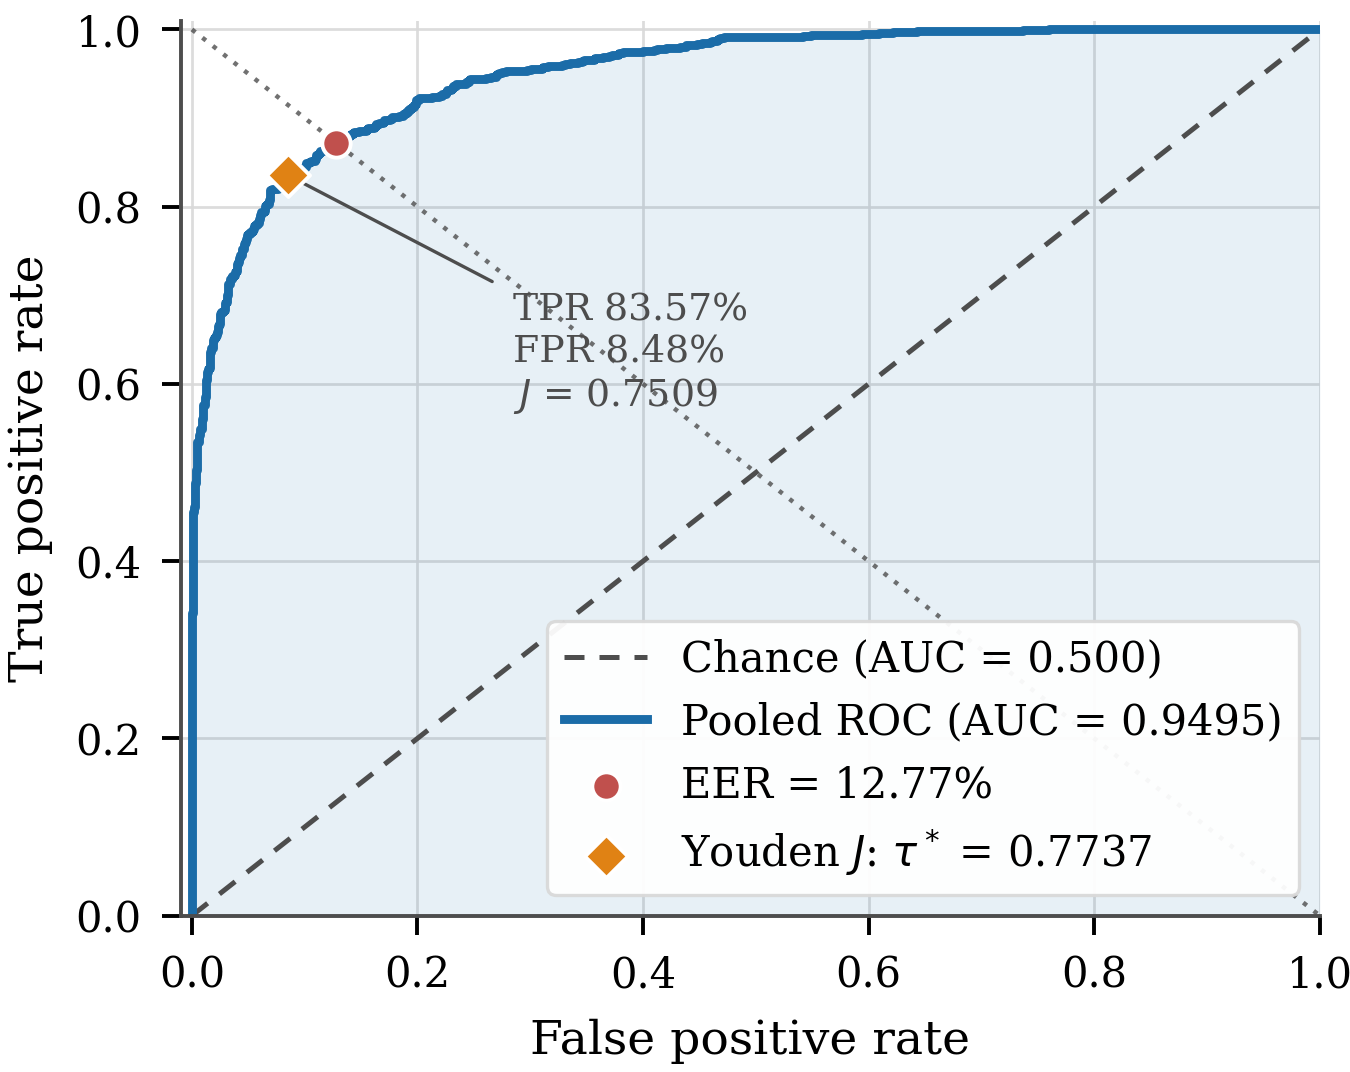
\includegraphics[height=2.45in]{fig_roc_pooled.png}\hfill
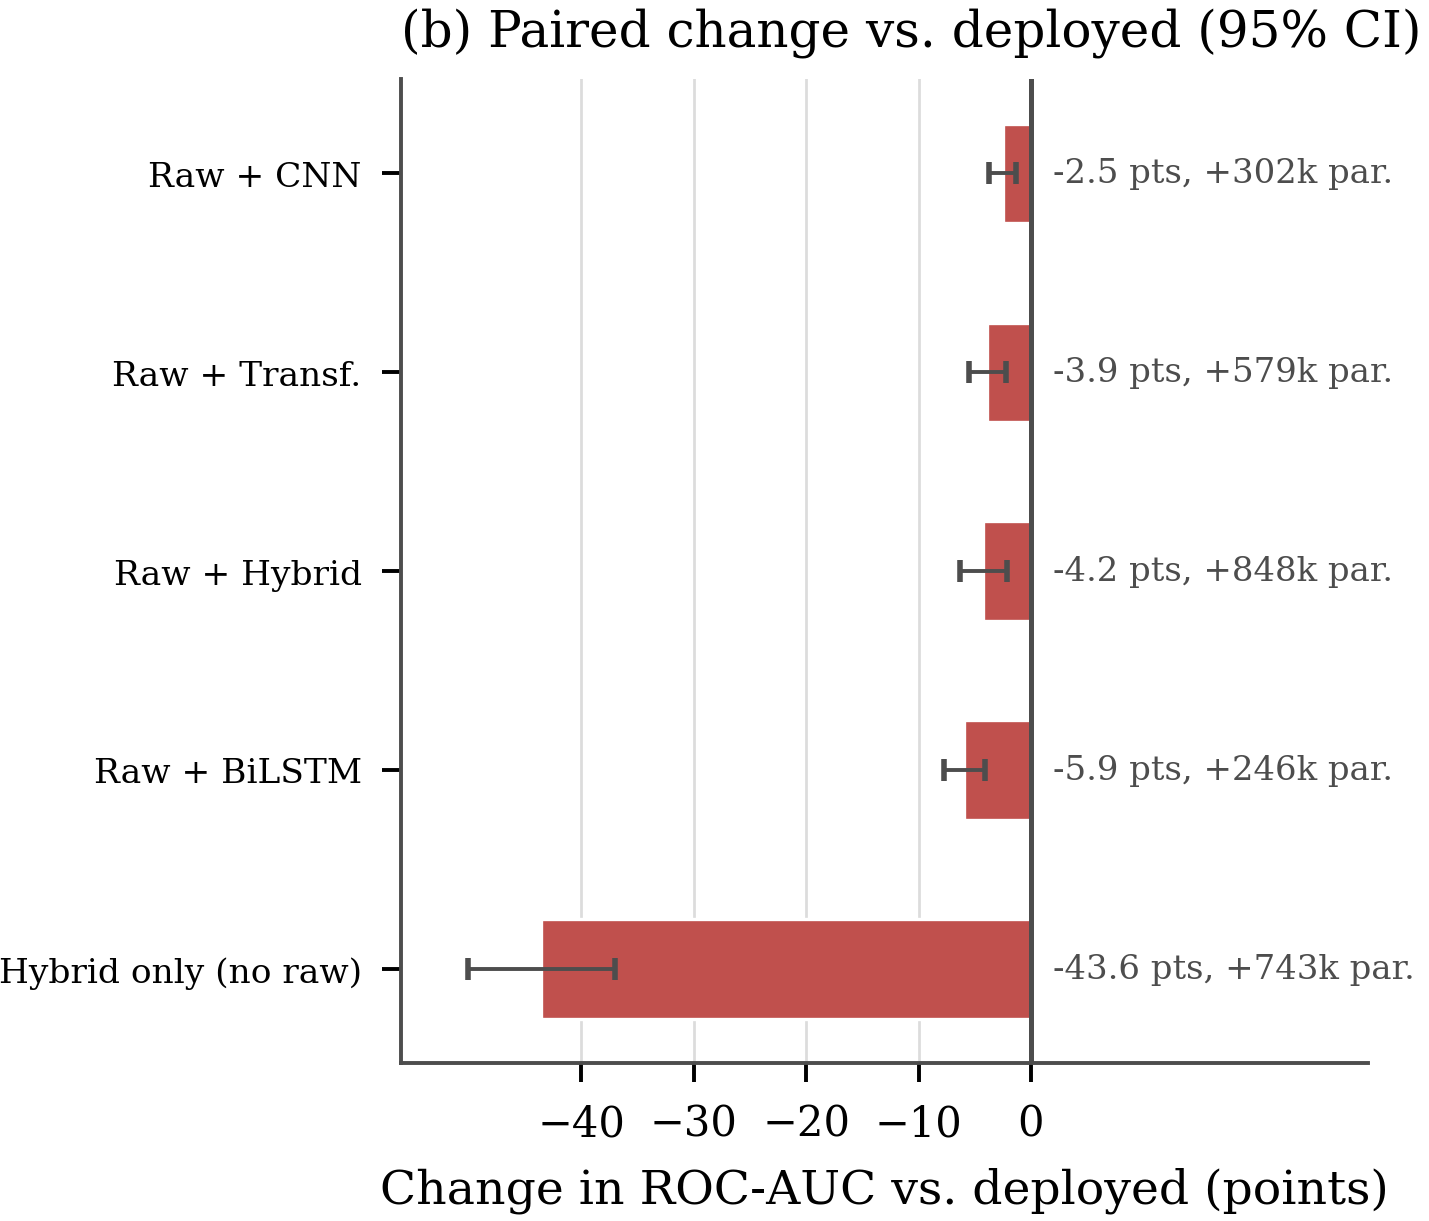
\includegraphics[height=2.45in]{fig_ablation_b.png}
\caption{Left: pooled ROC over all 2{,}240 leave-one-subject-out verification
pairs, with the equal-error point and the Youden-optimal point
$\tau^* = 0.7737$ marked. Right: paired change in ROC-AUC against the deployed
model for each ablation variant, with $95\%$ confidence intervals; every
interval lies wholly below zero.}
\label{fig:roc}
\end{figure*}

\subsection{Operating Points and Error Structure}

Fig.~\ref{fig:roc} (left) shows the pooled ROC; per-fold curves range from
Subject 13 ($0.985$) to Subject 12 ($0.870$), with an envelope that is narrow
mid-range but widens near the origin, so low-false-accept operation is where
subject identity matters most. At the native $\tau = 0.5$ the system produces
987 true positives, 962 true negatives, 158 false positives and 133 false
negatives ($87.01\%$ accuracy). The Youden-optimal $\tau^* = 0.7737$ moves 63
pairs from false-positive to true-negative at the cost of 51 additional false
negatives: false positives fall from 158 to 95, precision rises from $86.20\%$
to $90.79\%$ and recall falls from $88.12\%$ to $83.57\%$. Which is preferable is
a policy question; in forensic screening a false positive means accepting a
forgery, so the stricter threshold is the default. The $987/962/158/133$ matrix
is the $\tau = 0.5$ matrix and should not be quoted as the Youden one. Both
classes are strongly saturated---genuine median score $0.999$, impostor
$0.0007$---so only 86 pairs ($3.8\%$) lie between the equal-error and Youden
thresholds: threshold choice redistributes a small, hard residue, and reported
confidence values should not be read as calibrated probabilities.

\subsection{Architectural Ablation}
\label{sec:ablation-results}

The dual-path stack of Section~\ref{sec:aux} is inert in the deployed
checkpoint; the obvious question is whether it should be. Each of five
variants encodes both sequences with shared weights, preserves the
time axis, and forms the same per-timestep comparison tensor for the same
downstream CNN and classifier. The control, \emph{Raw}, uses an identity
encoder and reproduces the deployed model exactly at $133{,}058$ parameters.
Four \emph{Raw~+~X} variants concatenate the encoded comparison onto the raw
one, so each contains the deployed model's evidence and can only justify itself
by improving on it. \emph{Hybrid only} removes the raw comparison, isolating
what the encoder contributes alone.

The result is unambiguous and it is negative (Table~\ref{tab:ablation}, Fig.~\ref{fig:roc}, right). The
deployed model is the best of the five, at
$94.25\% \pm 3.09\%$ ROC-AUC. Because all variants share folds and seeds the
comparison is pairwise, removing fold difficulty and initialisation luck. The
paired deficits range from $-2.53$ points for \emph{Raw~+~CNN} to $-5.93$ for
\emph{Raw~+~BiLSTM}; all four are significant at $p < 10^{-3}$ (two-sided
paired $t$-test, $n = 39$), no variant wins more than 9 of its 39 paired
trials, and every $95\%$ CI lies wholly below zero. Adding capacity does not
merely fail to help: the largest variant, at $981{,}000$ parameters, is $4.22$
points worse than the $133{,}058$-parameter control.

\emph{Hybrid only} settles which half of the architecture carries the signal.
Stripped of the raw per-timestep comparison it reaches $50.70\% \pm 20.81\%$
ROC-AUC---indistinguishable from chance, with a standard deviation four times
any other variant's, indicating it often fails to learn at all. The
discriminative information is in the direct per-dimension comparison, where
dimension $j$ of each sequence is the same physical quantity and subtraction is
meaningful; passing both through a learned encoder first destroys that
correspondence and forces the classifier to recover it from what begins as a
random projection. The ablation thus justifies the deployed architecture: the
inert branch of Section~\ref{sec:aux} is not a missed opportunity, and a richer
temporal encoder is here a reliable regression, not a free improvement.

\begin{table}[!tb]
\caption{LOOCV Ablation over 13 Folds and 3 Seeds ($n = 39$ Paired
Observations per Variant). $\Delta$ is the Paired Change in ROC-AUC against the
Deployed Model}
\label{tab:ablation}
\centering
\footnotesize
\begin{tabular}{@{}lrrrr@{}}
\toprule
\tabhead{Variant} & \tabhead{Params} & \tabhead{ROC-AUC (\%)} &
\tabhead{Acc (\%)} & \tabhead{$\Delta$ AUC} \\
\midrule
Raw (deployed)     & 133{,}058 & $\mathbf{94.25 \pm 3.09}$ & $\mathbf{86.04}$ & --- \\
Raw + CNN          & 434{,}690 & $91.72 \pm 4.13$ & $82.66$ & $-2.53^{\ast}$ \\
Raw + Transformer  & 712{,}002 & $90.37 \pm 5.13$ & $80.32$ & $-3.88^{\ast}$ \\
Raw + Hybrid       & 980{,}994 & $90.03 \pm 6.11$ & $81.26$ & $-4.22^{\ast}$ \\
Raw + BiLSTM       & 379{,}074 & $88.32 \pm 6.08$ & $74.84$ & $-5.93^{\ast}$ \\
Hybrid only        & 876{,}162 & $50.70 \pm 20.81$ & $49.37$ & $-43.55^{\ast}$ \\
\bottomrule
\end{tabular}

\vspace{2pt}
\raggedright\footnotesize
$^{\ast}$Significant at $p < 10^{-3}$, two-sided paired $t$-test over the 39
matched (fold, seed) pairs. ``Hybrid only'' omits the raw comparison entirely.
\end{table}

\subsection{Face-Swap Video Validation}
\label{sec:deepfake-results}

Three face-swapped clips were generated as described in
Section~\ref{sec:setup}, pairing enrolled subjects so that both body and face
sources have enrolled signatures. Each clip was scored against the claimed
(face) identity at $\tau^* = 0.7737$ and re-scored against every enrolled
identity to find the closest match. All three were correctly rejected
(Table~\ref{tab:deepfake-video}): the claimed identity scores below
$0.006$---four to six orders of magnitude below $\tau^*$---while the true body
source scores above $0.9998$, exactly as Section~\ref{sec:threat} predicts. Pose
extraction succeeded over the full length of all three clips (135, 149 and 327
valid frames), so this is not an artefact of partial pose failure. One caveat:
for Subject~8\_body\_Subject~5\_face the correct match (Subject~8, $0.99999$) is
nearly tied by an impostor score for Subject~10 ($0.99986$), the two nearest
scores in the validation; the clip is still handled correctly, but the
embedding space is not uniformly well separated across subject pairs.

\begin{table}[!tb]
\caption{Face-Swap Video Validation ($n=3$; Existence Check, Not a
Statistically Powered Result)}
\label{tab:deepfake-video}
\centering
\small
\begin{tabular}{@{}lcccc@{}}
\toprule
\tabhead{Clip (body\_face)} & \tabhead{Claimed} & \tabhead{Sim.} &
\tabhead{Matched} & \tabhead{Sim.} \\
\midrule
Subj.6\_Subj.3 & Subj.\,3 & 0.0057 & Subj.\,6 & 0.9999 \\
Subj.7\_Subj.11 & Subj.\,11 & 0.0003 & Subj.\,7 & 0.9999 \\
Subj.8\_Subj.5  & Subj.\,5 & $<$0.0001 & Subj.\,8 & 0.99999$^{\ast}$ \\
\bottomrule
\end{tabular}

\vspace{2pt}
\raggedright\footnotesize
$^{\ast}$Nearest impostor score for this clip (Subject~10) was $0.99986$,
the closest margin observed; see discussion in text.
\end{table}

Three clips from a single pipeline under one masking configuration is an
existence check---not a statistically powered validation, silent on other
face-swap models, enhancement post-processing or heavier recompression, and
too small to establish how often near-collisions occur.

% ===========================================================================
\section{Explainability}
\label{sec:explain}

To determine what the verification network uses, we compute
gradient-times-input attribution on the 78-dimensional descriptor. For a sample
scored towards class $c$ we backpropagate the corresponding logit to the input
and take $A_{t,j} = \bigl| \hat{f}_{t,j} \cdot \partial\ell_c/\partial\hat{f}_{t,j} \bigr|$, aggregating over timesteps and over each joint's three coordinates, then
normalising to $[0,1]$, averaged over 26 samples (two per
identity)~\cite{sundararajan}. Because the gradient path runs through the
verification head, this describes the function that actually produces the
verdict.

\subsection{Joint-Level Attribution}

The left shoulder receives the highest attribution ($1.000$; Fig.~\ref{fig:joints}), followed by the right heel ($0.940$), left foot index ($0.931$) and left knee ($0.897$); both hips rank lowest ($0.665$ left, $0.566$ right).

The structure is biomechanically coherent: shoulders, carrying the trunk
countermotion that balances angular momentum during swing, and the distal foot
segments, registering heel strike and toe-off, dominate~\cite{perry_gait,winter_biomech},
while the hips rank lowest as expected, since the pelvis centre is the origin of
the coordinate normalisation. We do not over-interpret the left--right asymmetry: with 13 subjects and 26 samples it is as consistent with cohort-specific or viewpoint bias as with anything learned about laterality.

\begin{figure*}[!t]
\centering
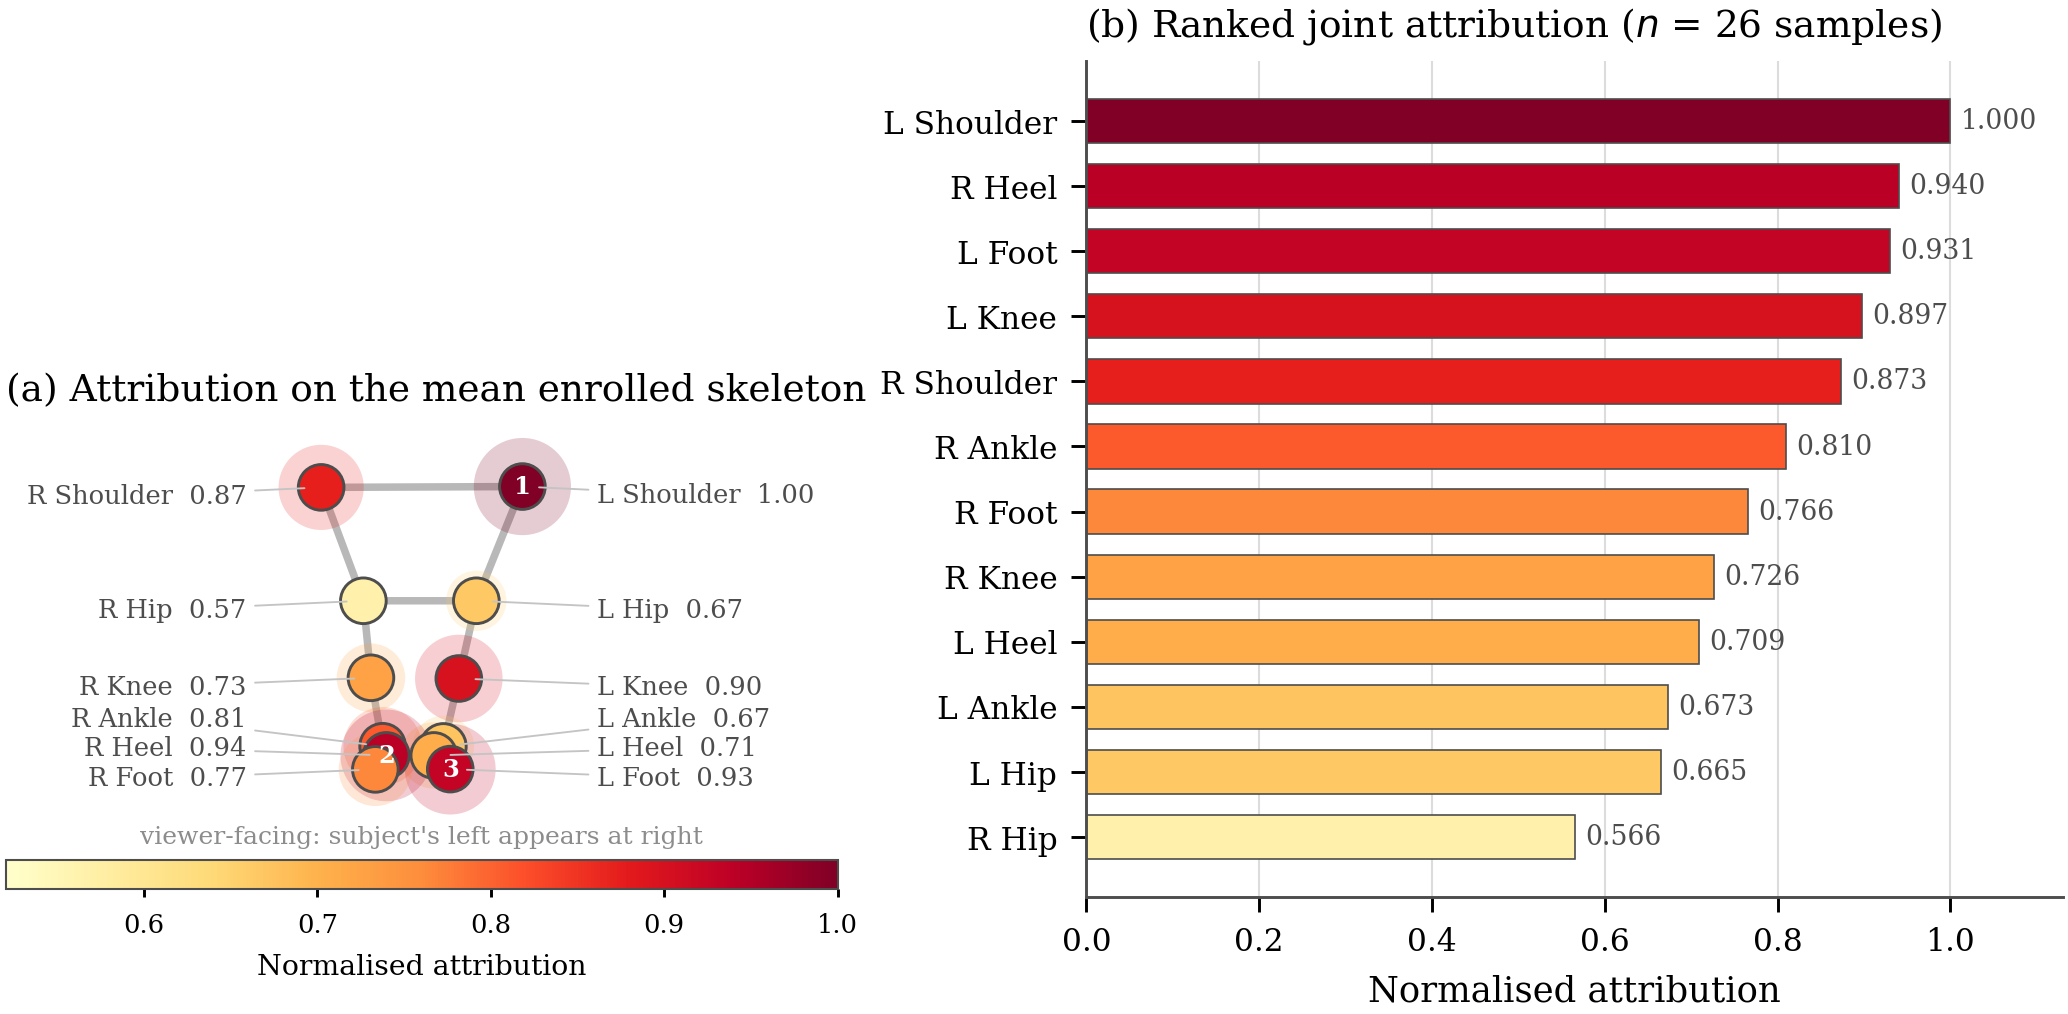
\includegraphics[height=1.25in]{fig10_joint_importance.png}
\caption{Joint-level attribution (a) on the mean enrolled skeleton and (b) ranked ($n=26$ samples).}
\label{fig:joints}
\end{figure*}

\subsection{Feature-Group Attribution}

\begin{figure}[!tb]
\centering
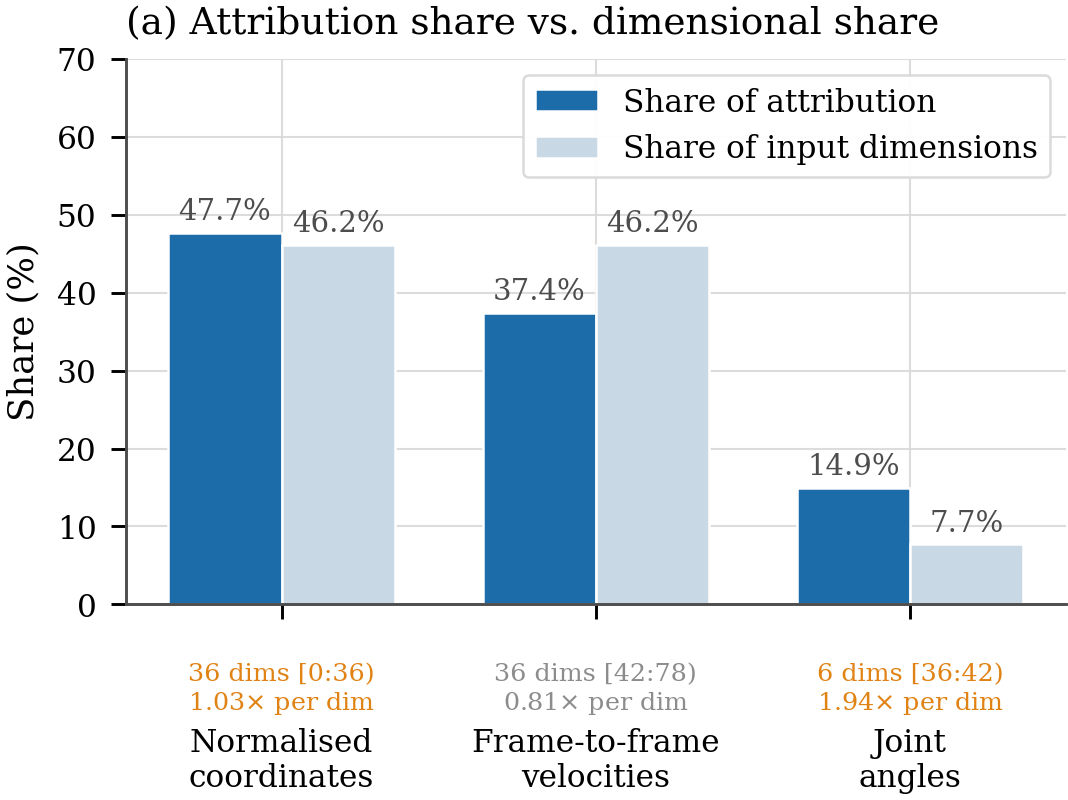
\includegraphics[width=0.86\columnwidth]{fig_groups_a.png}
\caption{Share of attribution against share of input dimensions for each
feature block. Joint angles occupy $7.69\%$ of the input but draw $14.92\%$ of
attribution, a per-dimension ratio of $1.94$.}
\label{fig:groups}
\end{figure}

Attribution decomposes by feature block as follows (Fig.~\ref{fig:groups}). Coordinates take $47.68\%$, velocities $37.40\%$ and joint angles $14.92\%$, against dimensional shares of $46.15\%$, $46.15\%$ and $7.69\%$: per-dimension ratios of $1.03$, $0.81$ and $1.94$. The six angle features are thus roughly twice as influential as the average coordinate and nearly two and a half times the average velocity. The six scale-free, rotation-invariant angles are the most information-dense part of the descriptor, suggesting a cheaper angle-weighted feature set may retain most of the discriminative power, relevant to embedded deployment. 

% ===========================================================================
\section{Discussion}
\label{sec:discussion}

\subsection{Comparative Positioning}

We deliberately report no head-to-head table: the figures quoted in Section~
ef{sec:related} each use a different corpus, protocol and task, and our $94.95\%$ is a leave-one-subject-out verification result on a 13-subject corpus collected by the authors. Tabulating them would invite a
ranking they cannot support; no claim of superiority is made. Gait evidence has begun to appear in forensic practice: a 2025 trade-press account reports a commercial analysis accepted in a European murder case where the face occupied roughly $10 	imes 5$ pixels~\cite{forensic_gait}, indicating institutional interest, not a validated standard (the sub-$0.1\%$ EER is a vendor figure).

\subsection{What This Approach Buys}

Four properties follow from the modality rather than the model.
\emph{Independence from synthesis quality}: the detector never observes the
manipulated region, so better face-swap fidelity does not degrade it, breaking
the arms-race coupling that constrains artefact-based
methods~\cite{recce,altfreezing}. \emph{Uncorrelated failure modes}: the
evidence is disjoint from that used by facial detectors, so the two families
fail on different inputs---making fusion natural not because gait is stronger
but because it is independent. \emph{Privacy}: video is reduced to 12 skeletal coordinates per frame, retaining no facial imagery (though gait is itself a biometric). \emph{Degradation profile}: gait stays recoverable at distances where facial analysis is not viable~\cite{forensic_gait}.

\subsection{Limitations and Threats to Validity}
\label{sec:threats}

We list these in descending order of how much they should temper the results.
\emph{The face-swap validation is small.} 3/3 clips were rejected with
true-source similarity above $0.9998$, but $n=3$ from one generator under one
masking configuration is an existence check that establishes no detection rate
or confidence interval; several dozen clips across at least two generators is the
most important gap. \emph{Thirteen subjects is a small cohort.} Augmentation
multiplies sequences, not gaits, so the effective sample is 13; LOOCV at this
size carries wide confidence intervals~\cite{varoquaux_small}, reflected in the
$\pm 3.08$ AUC and $\pm 6.82$ recall standard deviations, and CASIA-B-scale
validation is needed before these are treated as population estimates. The
cohort is also demographically narrow (students aged roughly 19--25;
age-related and pathological gait are unrepresented). \emph{The ablation is
specific to this scale.} Twelve training subjects is a regime that penalises
capacity, so the finding is not a general claim that temporal encoders cannot
help gait verification, and whether the ordering reverses on a CASIA-B-scale
cohort is untested. \emph{No standard-benchmark comparison.} We report no
FaceForensics++, Celeb-DF or DFDC figure: those corpora are face-centred and lack
the full-body walking this method requires. \emph{Conditions are controlled}:
indoor, cooperative, unobstructed full-body framing, two viewpoints; occlusion,
crowding, oblique angles, carried loads and varied footwear are unevaluated.
\emph{The threat model has a boundary.} A generator that re-synthesises, retimes
or warps whole-body motion violates its assumption; such systems exist and are
the subject of emerging benchmarks~\cite{ttdf,humanactionclips}, and current
generative animation appears not to preserve gait identity cues
faithfully~\cite{gaitfidelity}, which suggests---but does not show---that gait
may remain discriminative against full-body synthesis. \emph{Scope of the
verdict.} The system adjudicates a claimed identity, requires enrolment and
cannot flag a synthetic person claiming none; it is a verification component, not
a general-purpose detector, and its scores are not calibrated probabilities.

\subsection{Future Work}

Priorities: quantify detection on many more forgeries across multiple face-swap models, extend the cohort, and explore graph convolutional modelling~\cite{gaitgraph}, per-subject threshold calibration (Section~
ef{sec:perfold}) and an angle-weighted descriptor for embedded screening.

% ===========================================================================
\section{Conclusion}
\label{sec:conclusion}

We have presented a face-swap deepfake detector that verifies identity from
skeletal gait rather than facial artefacts, exploiting the fact that
face-region-only manipulation leaves the source body's locomotion intact. A
difference-based temporal convolutional network over 78-dimensional descriptors
from 12 MediaPipe landmarks attains a pooled ROC-AUC of $94.95\%$, accuracy of
$87.04\% \pm 3.65\%$ and an equal error rate of $12.27\% \pm 3.80\%$ across 13
leave-one-subject-out folds and 2{,}240 verification pairs; the minimal network
beats every encoder configuration tested, and stripping the raw comparison
reduces it to chance. The face-swap validation correctly rejected all three
clips (true-source similarity above $0.9998$) but remains an existence check on
a single generator, thirteen subjects is a small basis for generalisation, and
the ablation ordering is established at this cohort size only. Looking at what the adversary declines to model changes the terms of the problem, and body motion is, for now, exactly that.

\ifismanon\else
% ---------------------------------------------------------------------------
\section*{Acknowledgment}
We thank the volunteers who contributed walking recordings. GaitDeepfake-13 is
on IEEE DataPort (DOI: 10.21227/ngh5-b637); code at
\url{https://github.com/Arhaan-P/DeepFake-Detection}.
\fi

\bibliographystyle{IEEEtran}
\bibliography{ism_paper}

\end{document}
